



\begin{example2}{Beispiel DEA (eindeutig)} Sprache: $L(M)=\left\{1 x 1 \mid x \in\{0\}^{*}\right\}$
    
    \begin{minipage}{0.45\linewidth}
        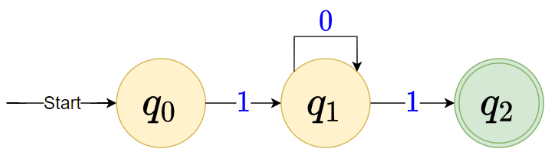
\includegraphics[width=1\linewidth]{images/dea_example.png}
    \end{minipage}
    \hspace{1mm}
    \begin{minipage}{0.5\linewidth}
        \textbf{Konfiguration} auf $\omega=101$
        \begin{itemize}
        \item Startkonfiguration $\rightarrow\left(q_{0}, 101\right)$
        \item Endkonfiguration $\rightarrow\left(q_{2}, \varepsilon\right)$
        \end{itemize}
    \end{minipage}

    \textbf{Berechnung}

    \resizebox{\linewidth}{!}{
    $\omega=101 \rightarrow\left(q_{0}, 101\right) \vdash_{M}\left(q_{1}, 01\right) \vdash_{M}\left(q_{1}, 1\right) \vdash_{M}\left(q_{2}, \varepsilon\right) \rightarrow \text{akzeptierend}$\\
    }

    \resizebox{\linewidth}{!}{
    $\omega=10 \rightarrow\left(q_{0}, 10\right) \vdash_{M}\left(q_{1}, 0\right) \vdash_{M}\left(q_{1}, \varepsilon\right) \rightarrow \text{verwerfend}$
    }
\end{example2}

\begin{example2}{NEA (nicht eindeutig)} Sprache: $L(M)=\left\{x 01 \mid x \in\{0,1\}^{*}\right\}$
    
    \begin{minipage}{0.55\linewidth}
        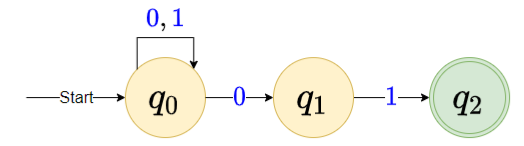
\includegraphics[width=1\linewidth]{images/nea_example1.png}
    \end{minipage}
    \hspace{1mm}
    \begin{minipage}{0.4\linewidth}
        \includegraphics[width=1\linewidth]{images/äquivalenter_nea.png}
        
        äquivalenter DEA
    \end{minipage}    
\end{example2}

\begin{remark}
    KA auf englisch: PDA = Push Down Automat
\end{remark}

\begin{KR}{Kellerautomat für kontextfreie Sprache} $\left\{0^{n} 1^{n} \mid n>0\right\}$
    \begin{itemize}
    \item $0,0 / 00 \quad$ Read $0 \quad$ Add $0 \quad(00-0)=0$
    \item $0, \$ / 0 \$ \quad$ Read 0 Add $0 \quad(\$ 0-\$)=0$
    \item $1,0 / \varepsilon$ Read 1 Remove 0 Read $(\varepsilon-0)=-0$
    \item $\varepsilon, \$ / \$ \quad$ Read $\varepsilon$ - $(\$-\$)=\varepsilon$
    \end{itemize}

    \begin{minipage}{0.5\linewidth}
        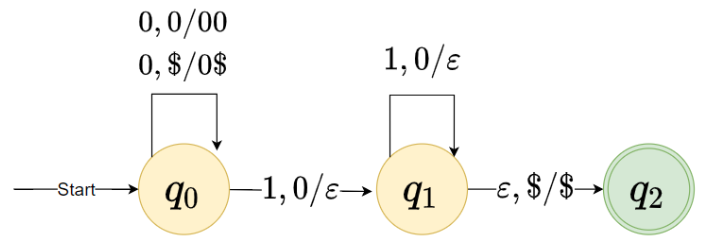
\includegraphics[width=1\linewidth]{kellerautomat_sprache.png}
    \end{minipage}
    \begin{minipage}{0.5\linewidth}
        $\omega_{1}=011:$

        \resizebox{\linewidth}{!}{
        $(q_{0}, 011, \$) \vdash(q_{1}, 11,0 \$) \vdash(q_{1}, 1, \$)$}
        $\rightarrow \omega_{1}$ verwerfend 
        
        Das Zeichen \$ zeigt an, dass der «Stack» leer ist.
    \end{minipage}
\end{KR}

\begin{concept}{NKA}Nichtdeterministischer KA für $\left\{\omega \omega^{R} \mid \omega \in\{0,1\}^{*}\right\}$\\
    
    \includegraphics[width=0.5\linewidth]{nka_übergangsfunktion.png}
\end{concept}

\begin{minipage}{0.5\linewidth}
    \begin{KR}{Loop (primitiv-rekursiv)}
        \begin{itemize}
            \item Zuweisungen:\\ $x = y + c$ und $x = y - c$
            \item Sequenzen: $P$ und $Q \rightarrow P; Q$
            \item Schleifen:\\ $P \rightarrow$ Loop $x$ do $P$ until End
        \end{itemize}
    \end{KR}
    
    \begin{example2}{Addition von natürlichen Zahlen}
    
        Add(x, y) = x + y
    \begin{lstlisting}[style=Pseudocode]
    LOOP x1 DO
        x2 = x2 + 1
    END
    x0 = x2 + 0
    \end{lstlisting}
    \end{example2}
\end{minipage}
\begin{minipage}{0.5\linewidth}
    \begin{KR}{While (Turing vollständig)}\\
        Erweiterung deer Sprache Loop
        \begin{itemize}
            \item While $x_i > 0$ do ... until End
        \end{itemize}
    \end{KR}
    
    \begin{example2}{Multiplikation \\von natürlichen Zahlen}
        
        Mul(x, y) = x * y
    \begin{lstlisting}[style=Pseudocode]
    WHILE x1 > 0 DO
        x1 = x1 - 1
        LOOP x2 DO
            x0 = x0 + 1
        END
    END
    \end{lstlisting}
    \end{example2}
\end{minipage}


\begin{example2}{Mehrband-Maschine}\\
    Spezifizieren Sie eine TM $M_{4}$, welche die Subtraktion von zwei natürlichen Zahlen $(a-b$, mit $a \geq b)$ realisiert.\\
    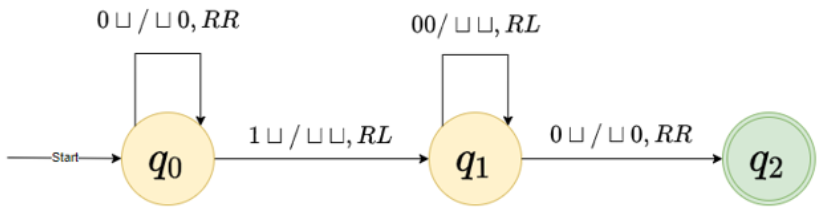
\includegraphics[width=0.5\linewidth]{mehrband_maschine1.png}\\
    Beispiel: $4-2=2$\\
    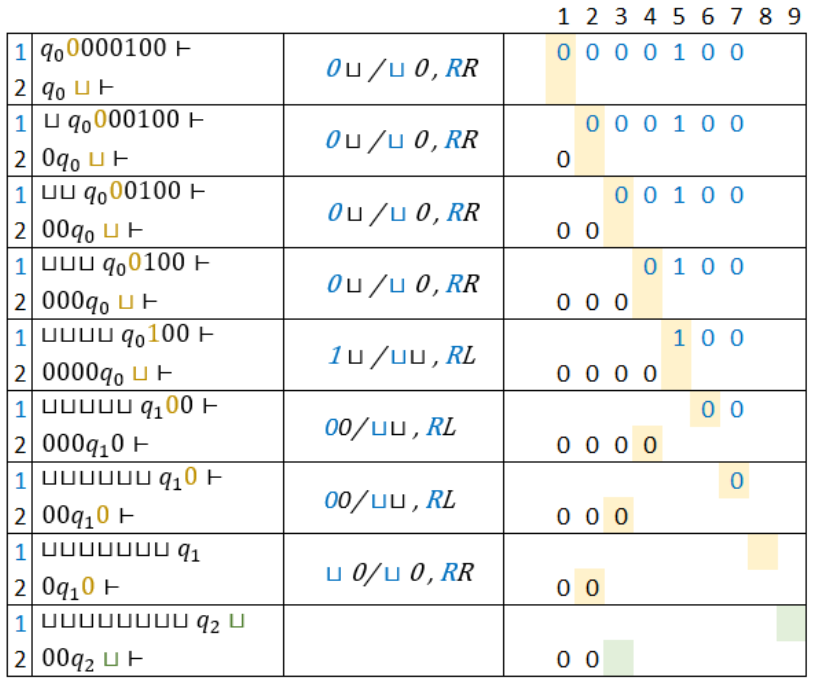
\includegraphics[width=1\linewidth]{mehrband_maschine2.png}
\end{example2}

\begin{KR}{GoTo (Turing vollständig)}
    \begin{itemize}
        \item Zuweisungen: $x_i = x_j + c$ und $x_i = x_j - c$
        \item Sprunganweisung: IF $x_i = c$ THEN GOTO $L_k$ ELSE GOTO $L_t$
        \begin{itemize}
            \item or simple: GOTO $L_k$
        \end{itemize}
        \item Schleifen: WHILE $x_i > 0$ DO ... HALT
    \end{itemize}
\end{KR}

\begin{example2}{Case distinction}
    \begin{lstlisting}[style=Pseudocode]
        M1: x0 = x3 + 0
        M2: IF x1 = 0 THEN GOTO M4
        M3: x0 = x2 +0
        M4: HALT
    \end{lstlisting}
\end{example2}

\subsubsection*{Übersicht}
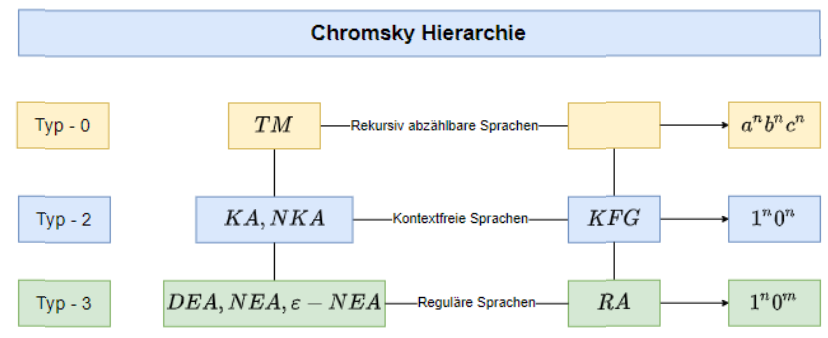
\includegraphics[width=0.8\linewidth]{chomsky_hierarchie.png}\\
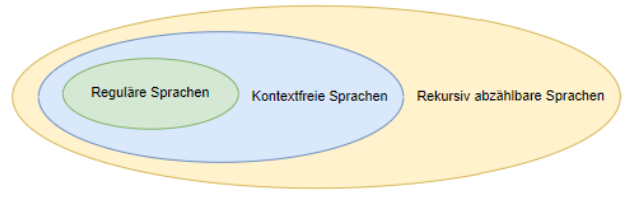
\includegraphics[width=0.5\linewidth]{sprachen.png}\\
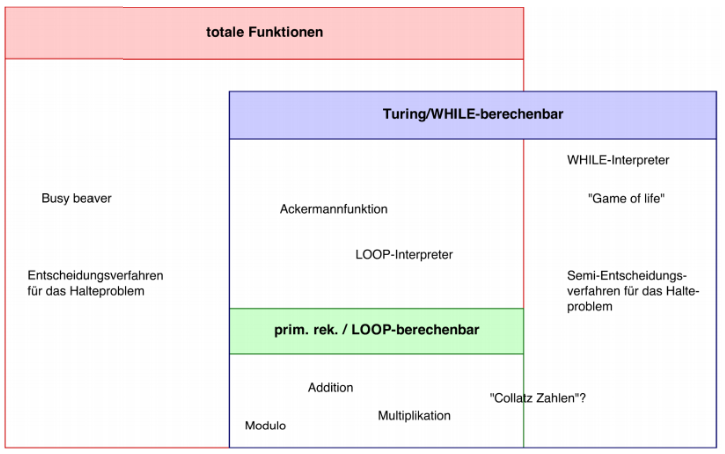
\includegraphics[width=1\linewidth]{funktionen.png}